\documentclass[14pt, a4paper]{report}
\usepackage{mathtext}
\usepackage[T2A]{fontenc}
\usepackage[utf8]{inputenc}
\usepackage[russian]{babel}
\usepackage{multirow}
\usepackage{slashbox}
\usepackage{makecell}
\usepackage{graphicx}
\usepackage{physics}
\usepackage{amstext}
\usepackage{caption}
\usepackage{subcaption}
\usepackage{cmap}
\usepackage{float}

\renewcommand{\thesection}{\arabic{section}.}
\renewcommand{\thesubsection}{\arabic{section}.\arabic{subsection}.}

\title{\textbf{Отчет о выполнении лабораторной работы 3.6.1 "Спектральный анализ электрических сигналов"}}
\author{Алпатова Александра, Калашников Михаил, Б03-205}
\date{}

\begin{document}
\maketitle

\textbf{Цель работы:}
изучить спектры сигналов различной формы и влияние параметров сигнала на вид соответствующих спектров; проверить справедливость соотношений неопределённостей; познакомиться с работой спектральных фильтров на примере RC-цепочки.
\newline

\textbf{В работе используются:}
\begin{itemize}
\item генератор сигналов произвольной формы
\item цифровой осциллограф с функцией быстрого преобразования Фурье
\end{itemize}

\section{Теоретическая справка}


\section{Экспериментальная установка}


\section{Проведение эксперимента}

\begin{enumerate}

\setcounter{enumi}{0}

\item Ознакомимся с устройством приборов.

\item Подключим один из выходов генератора к одному из каналов осциллографа и включим приборы в сеть.

\subsection{Исследование спектра периодической последовательности прямоугольных импульсов и проверка соотношений неопределённостей}

\item Настроим на генераторе генерацию прямоугольных импульсов с параметрами: $\nu_{повт}=1\ кГц$, $\tau=T/20=50\ мкс$.

\item Получим на осциллографе устойчивую картину сигнала.

\item Получим на осциллографе спектр сигнал, подобрав правильный масштаб по осям.

\item Определим как изменяется спектр при изменении параметров сигнала. При увеличении $\nu_{повт}$ уменьшается амплитуда спектра. При увеличении $\tau$ уменьшается полная ширина спектра.

\begin{figure}[H]
\centering
\includegraphics[scale=0.3]{images/361_1.png}
\caption{Измерение параметров последовательности прямоугольных импульсов}
\end{figure}

\item Проведем измерения амплитуды $a_n$ и частоты $\nu_n$ нескольких спектральных компонент и сравним значения с табличными.

\begin{table}[H]
\centering
\makebox[\textwidth][c] {
\begin{tabular}{| c | c | c | c | c | c |}
\hline
\hline
$n$ & 1 & 2 & 3 & 4 & 5 \\
\hline
$\nu_n^{эксп},\ кГц$ & 1.04 & 2.04 & 3.04 & 4.04 & 5.04 \\
$\nu_n^{теор},\ кГц$ & 1 & 2 & 3 & 4 & 5 \\
$|a_n|^{эксп},\ усл.\ ед.$ & 300 & 295 & 289 & 281 & 271 \\
$|a_n/a_1|^{эксп}$ & 1 & 0.99 & 0.97 & 0.94 & 0.90 \\
$|a_n/a_1|^{теор}$ & 1 & 0.98 & 0.96 & 0.94 & 0.90 \\
\hline
\end{tabular}
}
\end{table}

\item Фиксируя период, проведем измерения полной ширины спектра сигнала $\Delta\nu$.

\begin{table}[H]
\centering
\makebox[\textwidth][c] {
\begin{tabular}{| c | c | c | c |}
\hline
$\tau,\ мкс$ & 25 & 50 & 100 \\
\hline
$\Delta\nu,\ кГц$ & 80.6 & 40.1 & 20.1 \\
\hline
\end{tabular}
}
\end{table}

\item Зафикисируя длительность импульса, измерим растояния $\delta_\nu$ между соседними гармониками спектра.

\begin{table}[H]
\centering
\makebox[\textwidth][c] {
\begin{tabular}{| c | c | c | c |}
\hline
$T,\ мс$ & 1 & 2 & 3 \\
\hline
$\delta\nu,\ кГц$ & 1.99 & 1.03 & 0.60 \\
\hline
\end{tabular}
}
\end{table}

\item Построим графики зависимостей $\Delta\nu(1/\tau)$ и $\delta\nu(1/T)$ и заметим, что расхождения с теоретическими значениями минимальны.

\begin{figure}[H]
\centering
\makebox[\textwidth][c] {
\includegraphics[scale=0.6]{images/361_6.png}
}
\end{figure}

\subsection{Наблюдение спектра периодической последовательности цугов}

\item Настроим генератор на генерацию последовательных импульсов синусоидальной формы с параметрами $\nu_0=50\ кГц$, $T=1\ мс$, $N=5$. Получим на экране осциллографа устойчивую картину сигнала.

\item Получим на экране спектр сигнала и подберем масштаб для отображения полного спектра.

\item Изменяя параметры сигнала пронаблюдаем как изменяется наблюдаемый спектр.

\begin{figure}[H]
\centering
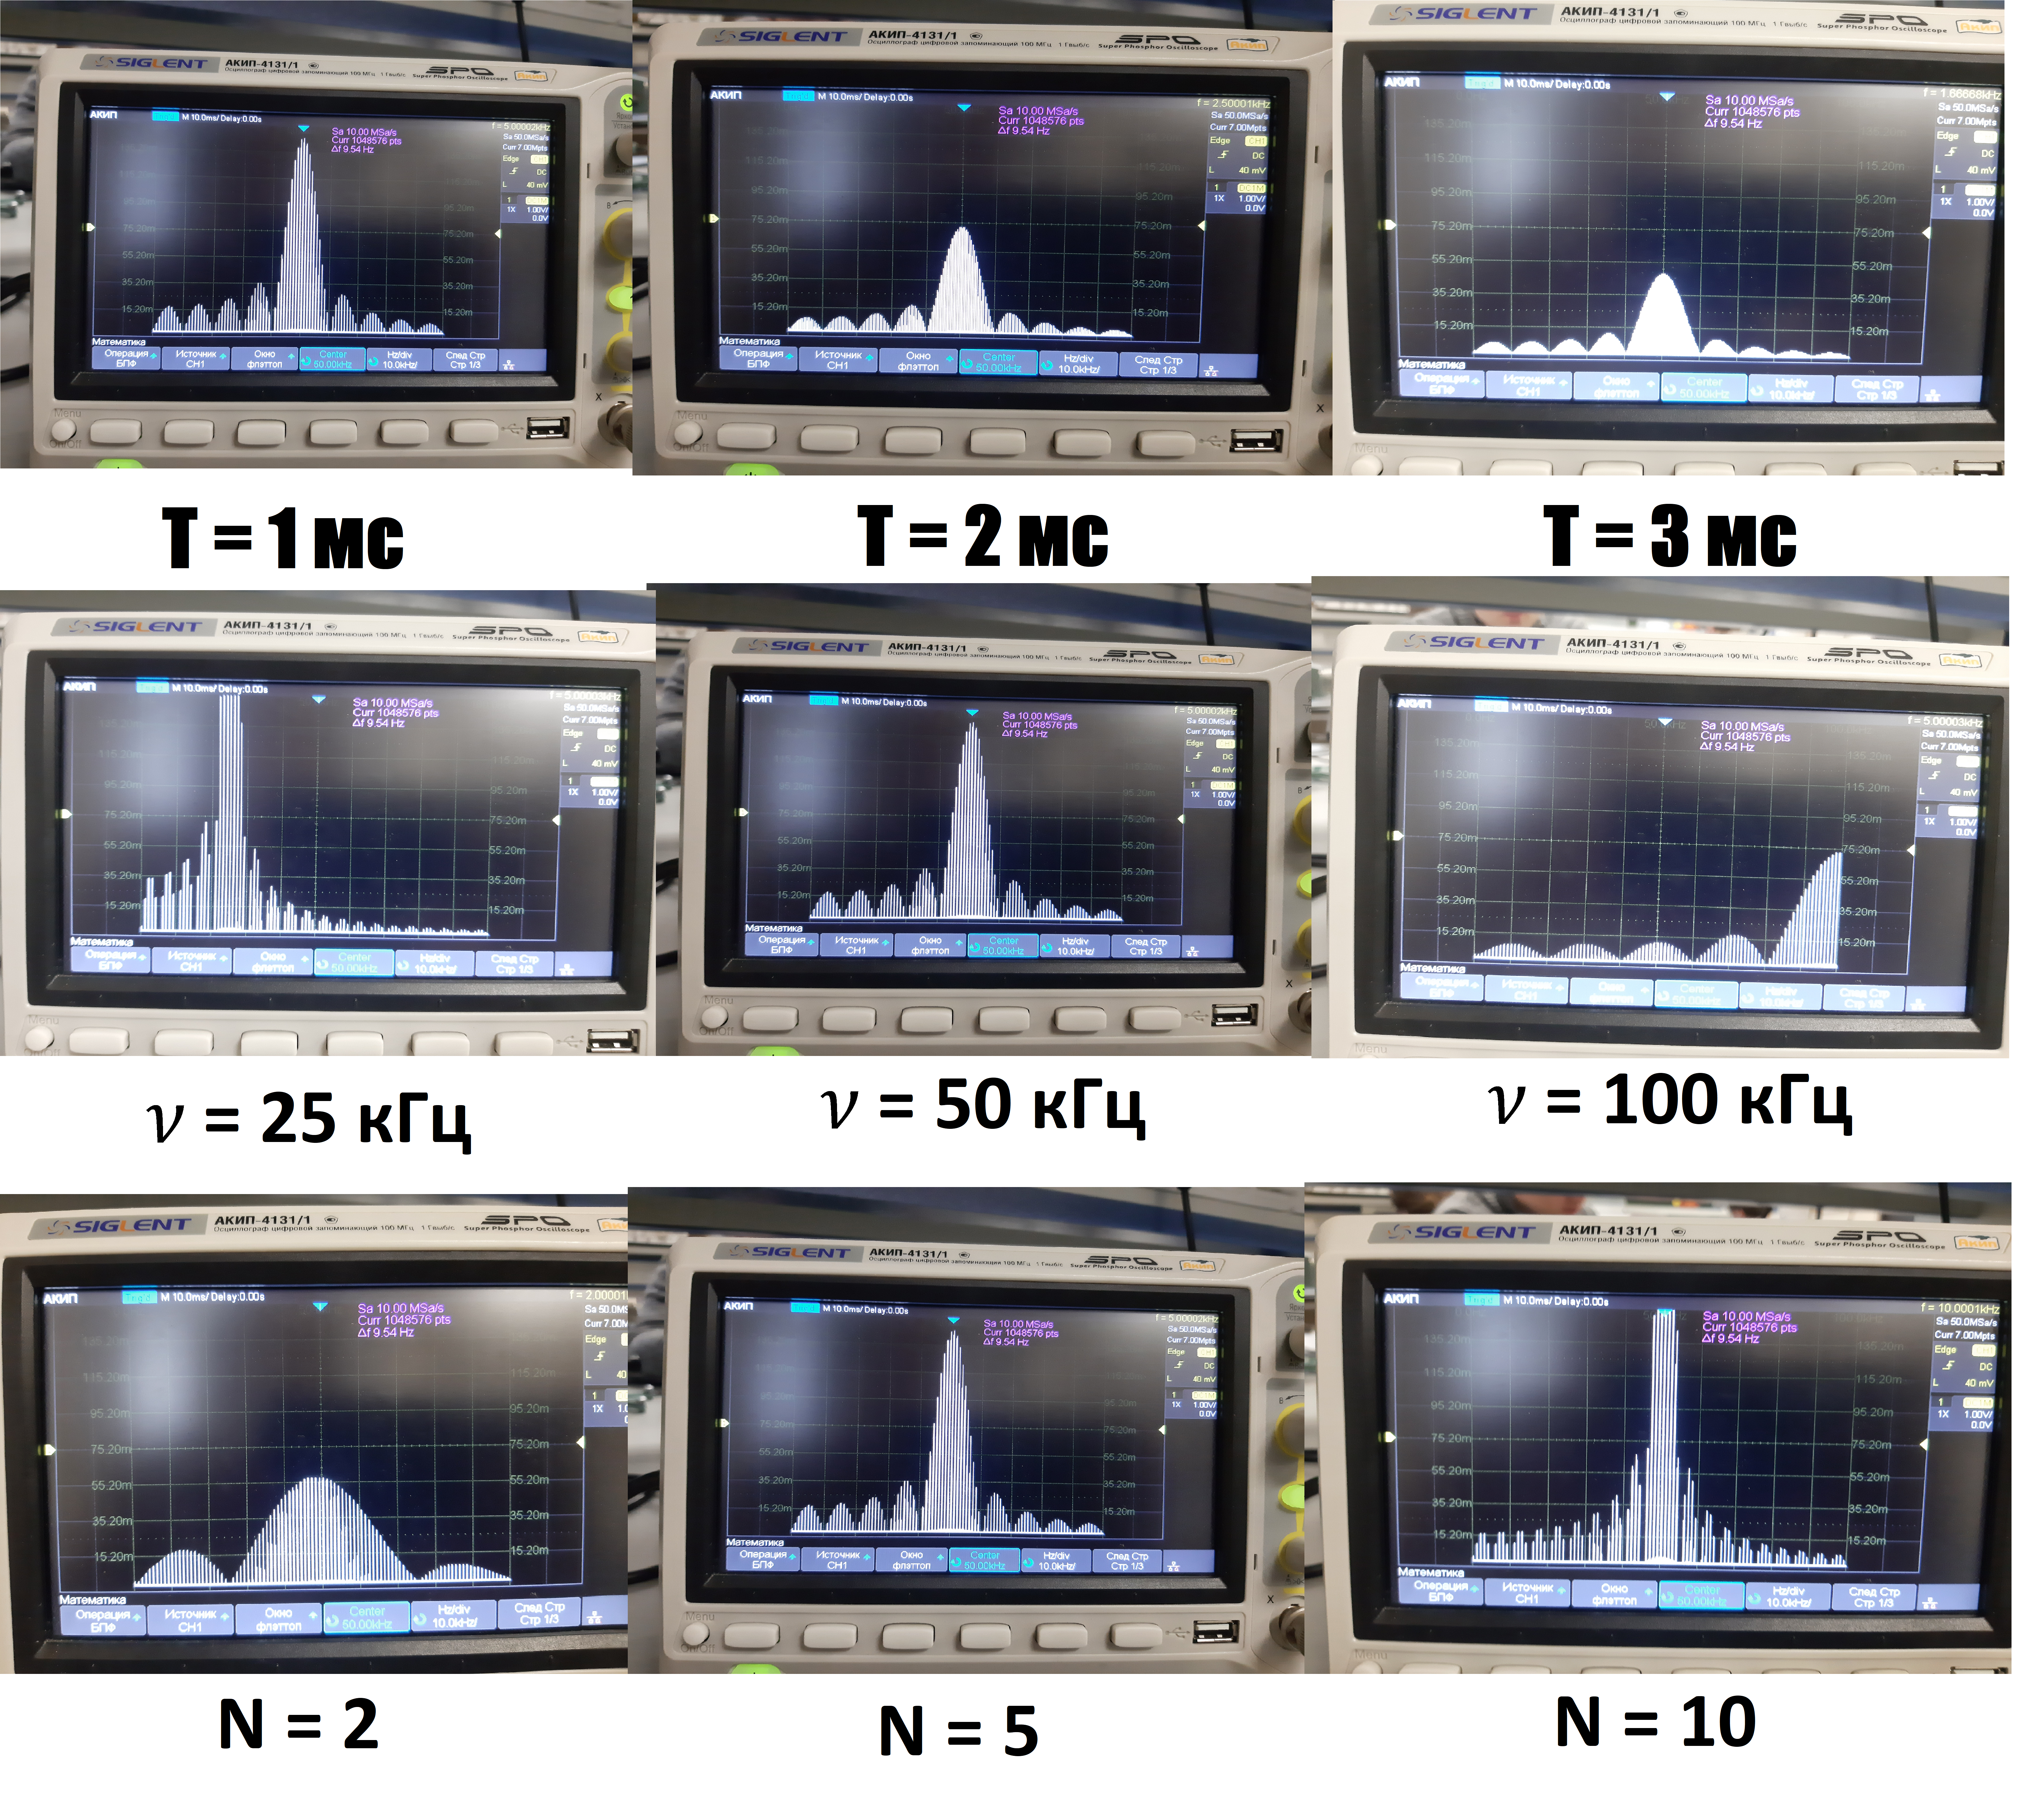
\includegraphics[scale=0.06]{images/361_2.png}
\caption{Изменение параметров последовательности цугов}
\end{figure}

\item Измерим ширину спектра $\Delta\nu$ и расстояние между гармониками $\delta\nu$. Убедимся в справедливости соотношения неопределенностей, проделав действия, описанные в пунктах 8-10. 

\begin{table}[H]
\centering
\makebox[\textwidth][c] {
\begin{tabular}{| c | c | c | c |}
\hline
$\nu,\ кГц$ & 25 & 50 & 100 \\
\hline
$\Delta\nu,\ кГц$ & 5.14 & 9.93 & 19.9 \\
\hline
$T,\ мс$ & 1 & 2 & 3 \\
\hline
$\delta\nu,\ кГц$ & 0.96 & 0.40 & 0.39 \\
\hline
\end{tabular}
}
\end{table}

\subsection{Исследование спектра амплитудно-модулированного сигнала}

\setcounter{enumi}{18}

\item Установим на генераторе режим модулированного по амплитуде синусоидального сигнала с параметрами $\nu_0=50\ кГц$, $\nu_{мод}=2\ кГц$, $m=0.5$. Получим на экране осциллографа устойчивую картину сигнала.

\item С помощью осциллографа измерим максимальную $A_{max}$ и $A_{min}$ амплитуды сигнала. Убедимся в справедливости равенства $m=\frac{A_{max}-A_{min}}{A_{max}+A_{min}}$.

\item Получим на экране спектр сигнала. С помощью осциллографа измерим частоты центральной и боковой гармоник. Пронаблюдаем как изменяется положение спектральных линий при изменении несущей частоты и частоты модуляции.

\begin{figure}[H]
\centering
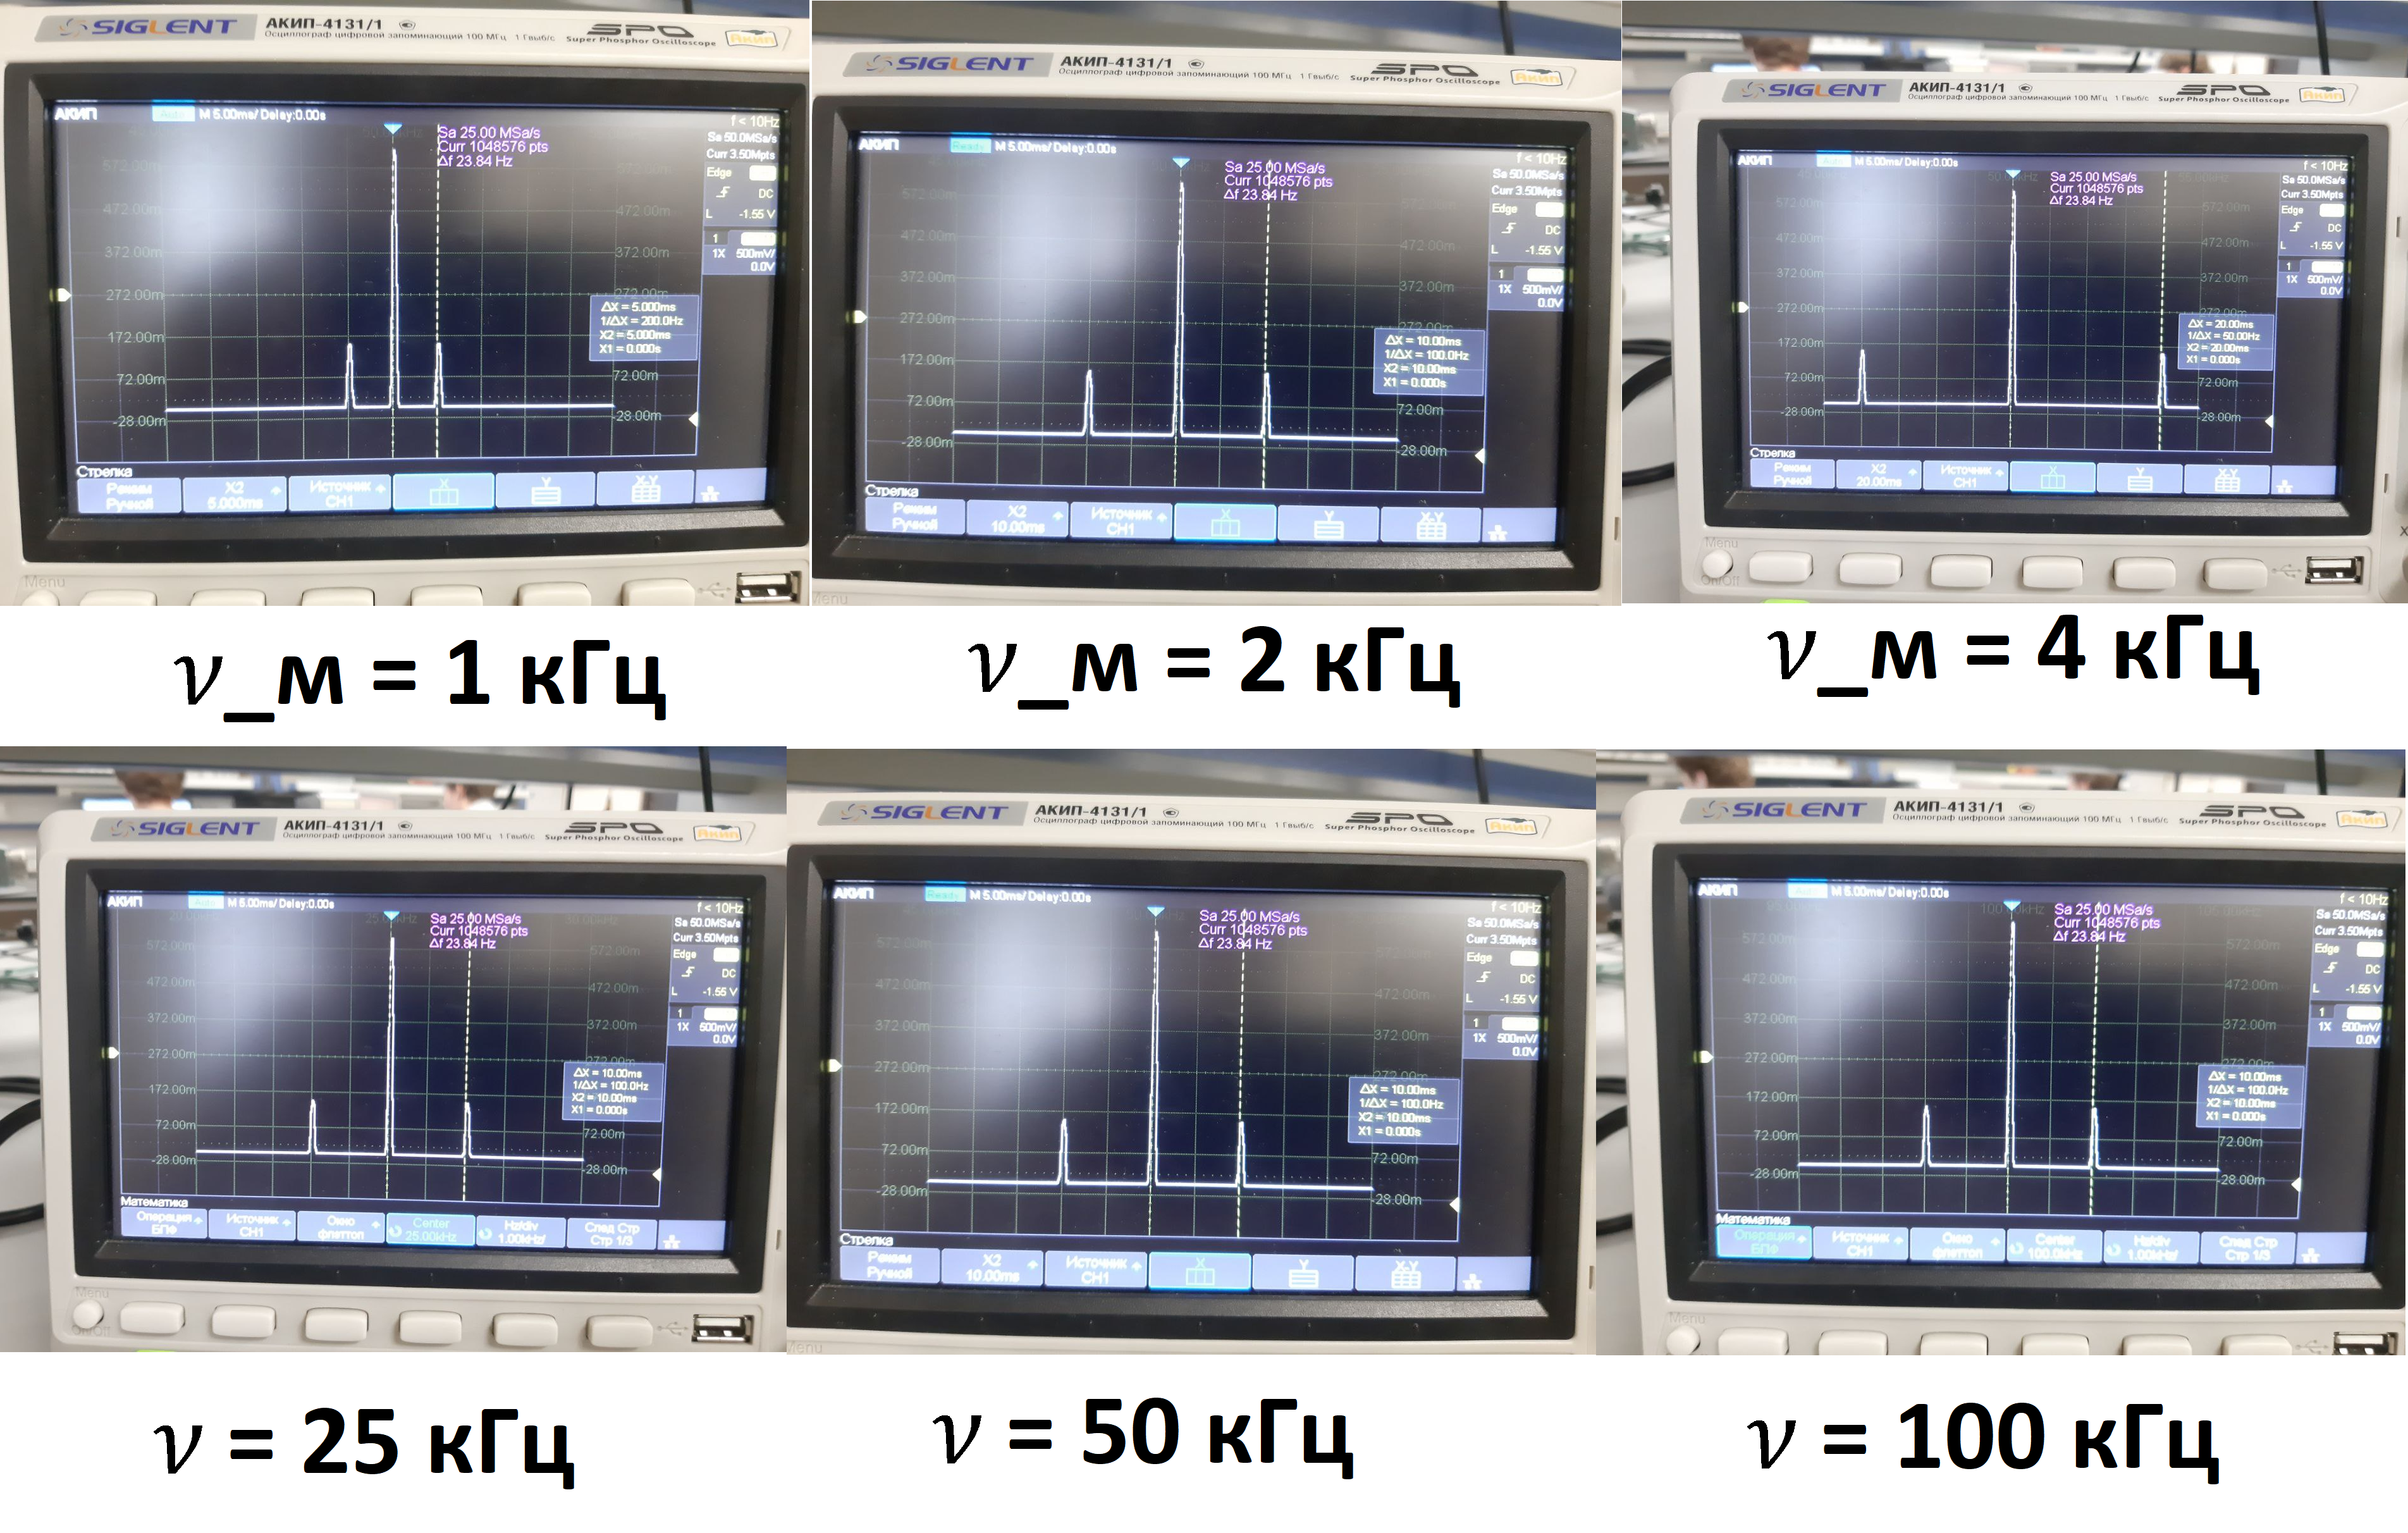
\includegraphics[scale=0.1]{images/361_3.png}
\caption{Изменение параметров последовательности амплитудно-модулированного сигнала}
\end{figure}

\item Изменяя глубину модуляции $m$ измерим отношение амплитуд боковой $a_{бок}$ и основной $a_{осн}$ спектральных линий.

\item Построим график зависимости $a_{бок}/a_{осн}$ от $m$.

\begin{figure}[H]
\centering
\includegraphics[scale=0.6]{images/361_4.png}
\caption{График зависимости $a_{бок}/a_{осн}$ от $m$}
\end{figure}

Полученные данные сходятся с теоретической зависимостью


\subsection{Исследование фильтрации сигналов}

\setcounter{enumi}{25}

\item Для $RC$-цепочки рассчитаем ее характерное время $\tau_{RC}=RC=3\ мкс$ и соответствующую частоту $\nu_{RC}=1/\tau_{RC}=333\ кГц$. Соберем схему и подадим на вход последовательность прямоугольных импульсов с периодом повторения $T\sim\tau_{RC}$ и длительностью $\tau\sim T/20$.

\item Пронаблюдаем спектр на выходе $RC$-цепочки при различных значениях периода повторения $T$.

\begin{figure}[H]
\centering
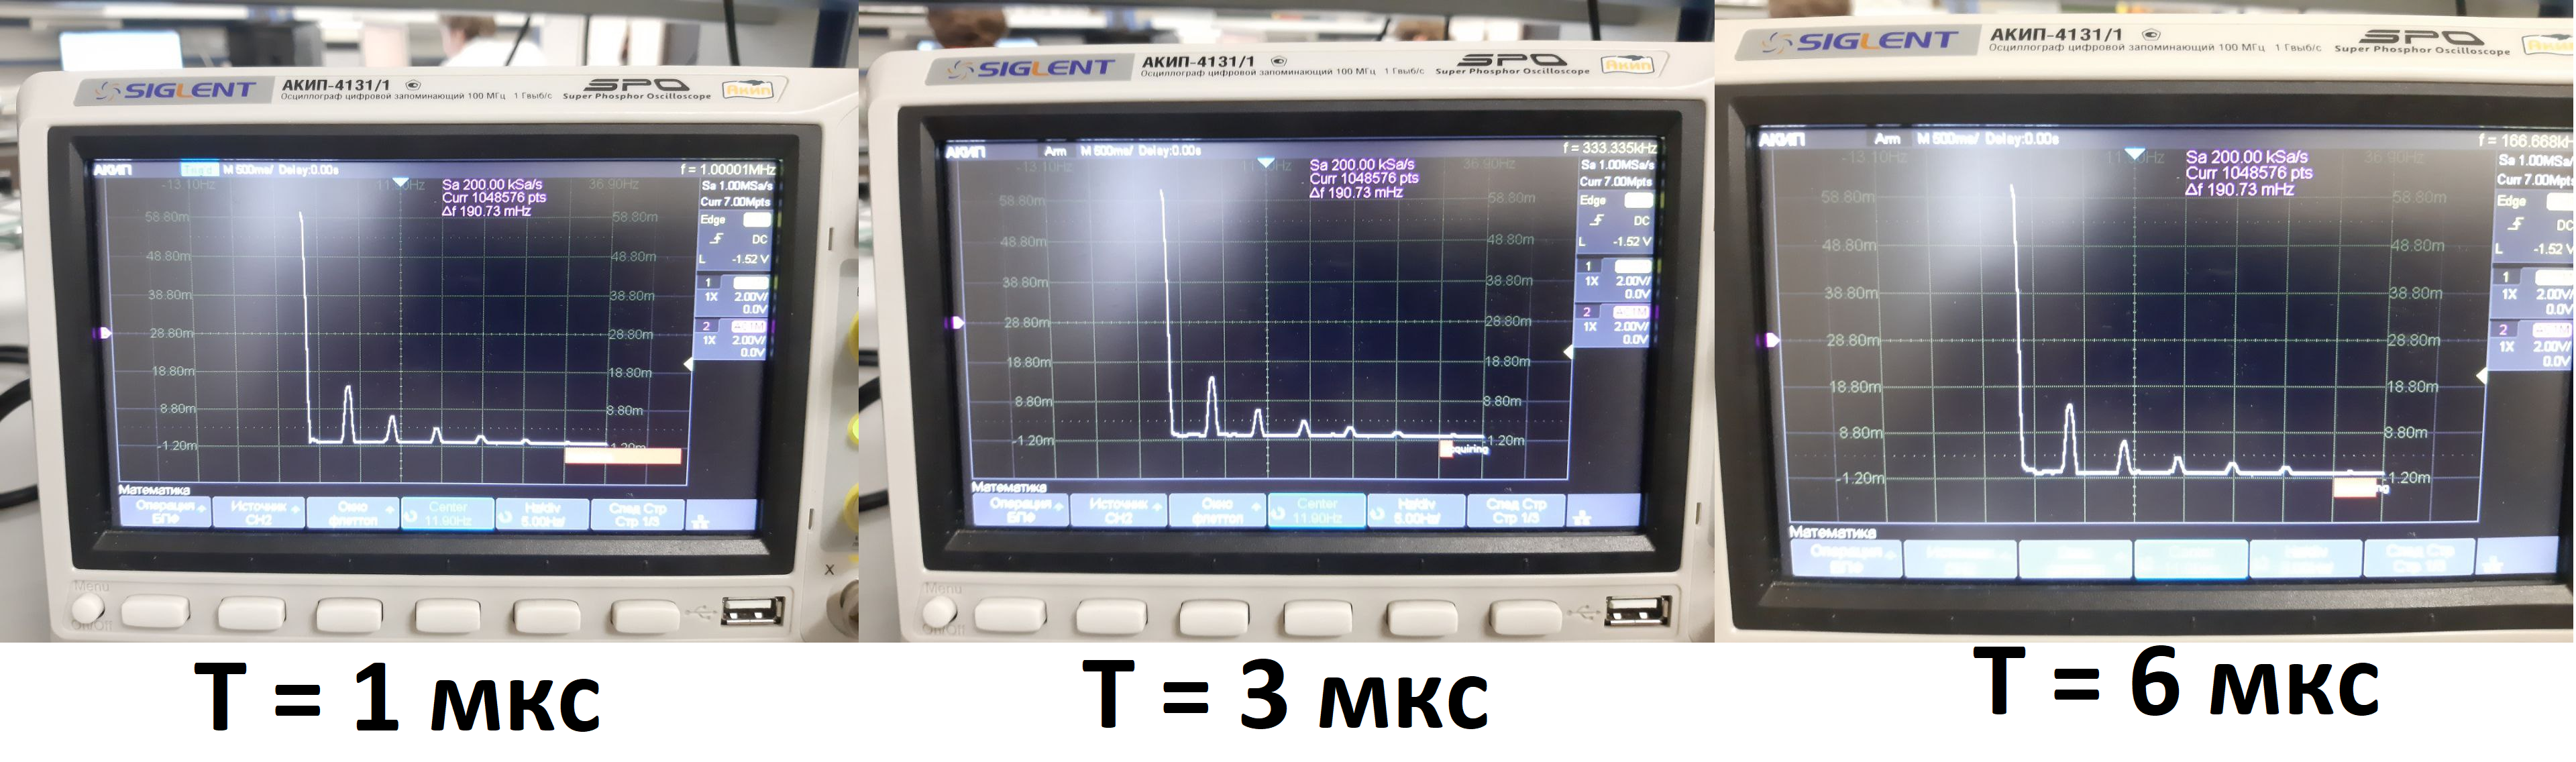
\includegraphics[scale=0.1]{images/361_5.png}
\caption{Спектр фильтрованного сигнала при различных значениях периода повторения}
\end{figure}

\item Проведем измерения отношений амплитуд соответствующих спектральных гармоник фильтрованного и исходного сигналов: $K_n=|a_n^ф|/|a_n^0|$.

\item Построим график зависимости амплитудного коэффициента фильтрации $K(\nu)$ от частоты $\nu=n\nu_0$. По полученной зависимости определим временную постоянная $RC$-цепочки $\tau_{RC}$. Также определим теоретическую зависимость $K_n(\nu)$. Известно, что после фильтрации: \[g(t)=\frac{1}{\tau_{RC}}\int_0^tf(t^\prime)dt^\prime\]. Найдем спектр такой функции при $T=\tau_{RC}$, $\tau=\tau_{RC}/20$, $k=2\pi\nu$:
\[|a_n^ф|=\frac{1}{\tau_{RC}^2}\left|\int_{-\frac{\tau}{2}}^{\frac{\tau}{2}}\int_0^tf(t^\prime) e^{-in\omega_0t}dt^\prime dt\right|=\frac{1}{\tau_{RC}^2}\left|\int_{-\frac{\tau}{2}}^{\frac{\tau}{2}}te^{-in\omega_0t}dt\right|=\]
\[=\frac{\pi\nu\tau\cos{\pi\nu\tau}-\sin{\pi\nu\tau}}{2(\pi\nu\tau_{RC})^2}\]
Спектр $a_n^0$ изначальной функции $f(t)$ нам известен: $|a_n^0|=\frac{\sin{\pi\nu\tau}}{\pi\nu\tau_{RC}}$. Найдем $K_n$:

\[K_n=\frac{|a_n^ф|}{|a_n^0|}=\frac{\pi\nu\tau\cos{\pi\nu\tau}-\sin{\pi\nu\tau}}{2(\pi\nu\tau_{RC})^2}\cdot\frac{\pi\nu\tau_{RC}}{\sin{\pi\nu\tau}}=\frac{\tau}{2\tau_{RC}}\left(\ctg{\pi\nu\tau}-\frac{1}{\pi\nu\tau}\right)\]

\end{enumerate}

\end{document}